\documentclass{beamer}

\mode<presentation>
{
  \usetheme{Madrid}      % or try Darmstadt, Madrid, Warsaw, ...
  \setbeamertemplate{navigation symbols}{}
  \setbeamertemplate{caption}[numbered]
} 

\colorlet{beamer@blendedblue}{black}

\usepackage[french]{babel}
\usepackage[utf8]{inputenc}
\usepackage[T1]{fontenc}
%\usepackage[squaren,cdot]{SIunits}
\usepackage{graphicx}
\usepackage{listings}
\usepackage{wrapfig}

\graphicspath{}

\logo{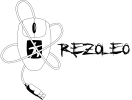
\includegraphics[height=0.8cm]{../../rezoleo.png}\vspace{10pt}\hspace{20pt}}
\title{Introduction aux réseaux}
\author{LEDER "Ziman" Simon}
\institute{Rezoleo\\}
\date{\today}

\begin{document}
	
	\maketitle

	\begin{frame}
		\frametitle{Sommaire} 
		\tableofcontents
	\end{frame}

\section{Topologie}

	\begin{frame}{Topologie}{Topologie en bus}
		\begin{wrapfigure}{r}{0.5\textwidth} 
			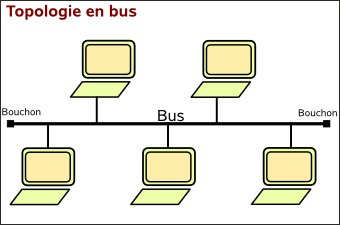
\includegraphics[scale = 0.7]{Bus.jpg}\\ 
			La Topologie en Bus : On dit qu’un réseau a une topologie en bus quand toutes les stations sont reliées à un câble unique.
		\end{wrapfigure}
	\end{frame}

	\begin{frame}{Topologie}{Topologie en anneau}
		\begin{wrapfigure}{r}{0.5\textwidth} 
			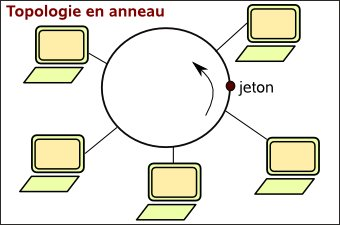
\includegraphics[scale = 0.7]{Anneau.jpg}\\
			La Topologie en Boucle (Anneau) : Un réseau a une topologie en anneau quand toutes ses stations sont connectées en chaîne les unes aux autres par une liaison bipoint et la dernière à la première. Une station reçoit une trame, la ré émet à la station successeur (avec un léger retard).
		\end{wrapfigure}
	\end{frame}

	\begin{frame}{Topologie}{Topologie en étoile}
		\begin{wrapfigure}{l}{1.0\textwidth} 
			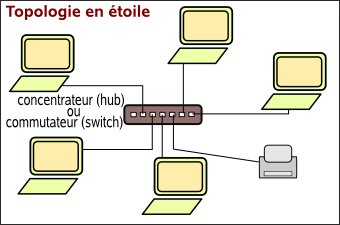
\includegraphics[scale = 0.7]{Etoile.jpg}\\
			La Topologie en Étoile : Un réseau à une topologie en étoile quand les stations sont raccordées par des liaisons point-à-point à des noeuds qui sont chargés de ré-émettre les trames.
		\end{wrapfigure}
	\end{frame}

\end{document}